\documentclass[sigconf,screen]{acmart}

\usepackage{tikz}
\usetikzlibrary{positioning}

\usepackage{xcolor}
\definecolor{blue}{cmyk}{1,0.8,0,0}
\definecolor{console}{cmyk}{0,1,0.9,0.25}

\usepackage{listings}
\lstdefinelanguage{pseudocode}[]{}{%
    basicstyle=\fontsize{8}{8}\selectfont\ttfamily,
    keywords={while,for,in,if,else,is,not,true,false,continue}
}
\lstdefinelanguage{console}[]{}{%
    basicstyle=\color{console}\fontsize{8}{8}\selectfont\ttfamily
}
\lstdefinelanguage{SaC}[]{}{%
    keywords={int,float,bool,inline,return,dim,shape,genarray,reshape,iota,take,drop,floor,add,sel,guard,abort},
    otherkeywords={->,|},
    morecomment=[s]{int[}{]},
    morecomment=[s]{float[}{]}
}
\lstset{%
    language=SaC,
    basicstyle=\fontsize{8}{8}\selectfont\ttfamily,
    keywordstyle=\color{blue},
    commentstyle=\color{blue},
    showstringspaces=false,
}

\newcommand{\tpdot}{\texttt{\textbf{.}}}
\newcommand{\tpplus}{\texttt{+}}
\newcommand{\tpstar}{\texttt{*}}
\newcommand{\tpnum}{\texttt{n}}
\newcommand{\tpnumshp}[2][\texttt{n}]{#1\texttt{:}#2}
\newcommand{\tpidshp}[2]{#1\texttt{:}#2}
\newcommand{\rest}{\ensuremath{tl}}
\newcommand{\atp}[4]{\ensuremath{\texttt{ATP}(#1,\,#2,\,#3,\,#4)}}
\newcommand{\fshp}{\texttt{kshp}}
\newcommand{\fdim}{\texttt{kdim}}
\newcommand{\vdim}{\texttt{vdim}}
\newcommand{\gtc}[4]{\ensuremath{\texttt{GTC}(#1\,v,\,#2,\,#3,\,#4)}}
\newcommand{\cdim}{\texttt{cdim}}
\newcommand{\deps}{\texttt{deps}}
\newcommand{\cenv}{\ensuremath{\sigma{}}}
\newcommand{\envmap}[3]{\ensuremath{[#1\mapsto\langle{}#3,\,#2\rangle{}]}}

\title{Type Patterns: Pattern Matching on Shape-Carrying Array Types}

\author{Jordy Aaldering}
\email{Jordy.Aaldering@ru.nl}
\affiliation{%
    \institution{Radboud University}
    \city{Nijmegen}
    \country{Netherlands}
}
\author{Sven-Bodo Scholz}
\email{SvenBodo.Scholz@ru.nl}
\affiliation{%
    \institution{Radboud University}
    \city{Nijmegen}
    \country{Netherlands}
}
\author{Bernard van Gastel}
\email{Bernard.vanGastel@ru.nl}
\affiliation{%
    \institution{Radboud University}
    \city{Nijmegen}
    \country{Netherlands}
}

\copyrightyear{2023}
\acmYear{2023}
\setcopyright{rightsretained}
\acmConference[IFL 2023]{The 35th Symposium on Implementation and Application of Functional Languages}{August 29--31, 2023}{Braga, Portugal}
\acmBooktitle{The 35th Symposium on Implementation and Application of Functional Languages (IFL 2023), August 29--31, 2023, Braga, Portugal}\acmDOI{10.1145/3652561.3652572}
\acmISBN{979-8-4007-1631-7/23/08}

\begin{document}

\begin{abstract}
In this paper we present type patterns: a notation for shape-carrying array types that enables the specification of dependent type signatures while maintaining flexibility and a high level of code readability.
Similar notations pre-exist, but we extend them to support rank-polymorphism and specifications of arbitrarily complex constraints between values and types.
Furthermore, we enable type patterns to double as a pattern matching mechanism against shapes and shape-components of array arguments, making those values directly available in the corresponding function bodies.

While this notation could be used as a basis for a dependently typed language, in our prototypical implementation in the context of SaC we do not require all dependencies to be resolved statically.
Instead, we follow a hybrid approach:
we map the proposed type patterns into the pre-existing type system of SaC, and we generate additional constraints which we try to statically resolve as far as possible by means of partial evaluation.
Any remaining constraints are checked at run-time.
We outline our implementation in the context of the SaC ecosystem, and present several examples demonstrating the effectiveness of this hybrid approach based on partial evaluation.
\end{abstract}
\keywords{Array Programming, Single assignment C, Rank-Polymorphism, Hybrid Types, Dependent Types, Type Constraints, Partial Evaluation, Pattern Matching, Shape Pattern, Type Pattern}


\maketitle

\section{Introduction}

Array programming languages play a crucial role in a wide range of data-centric applications, where the manipulation of multi-dimen\-sional arrays is at the core of many computational tasks.
In this domain, understanding and controlling the rank and shape of arrays is crucial, as they directly influence the correctness and efficiency of algorithms.

While array languages traditionally strive for universal applicability of operators to arrays of arbitrary rank and shape, some minimal restrictions on argument domains are usually inevitable, be it to avoid out-of-bound accesses, or to ensure some other structural consistency.
Unfortunately, the nature of these constraints is typically not only related to ranks and shapes of arguments alone, but to the values of arguments and return types as well.
The most prominent example for such a situation is element selection, which requires the index argument to have a value that is within the bounds of the shape of the array argument.

Using advanced type systems to provide static guarantees for such domain restrictions is highly desirable.
It makes these constraints explicit, provides the means to mechanically identify violations of them, and it opens the door for better code optimisation.
The value-dependent nature of these constraints, in the context of array programming languages, has led to several different type systems~\cite{indexed, cube, dependent-types, futhark-size-parameters, remora} that try to balance the trade-offs between readability of code, decidability of the type system, and expressiveness of the language.
Although most of these approaches prioritise decidability, in this paper we take a different approach.
Rather than starting out from a type system, we start out from a notation for domain constraints that aims at programming productivity.
Readability of domain constraints without any restrictions in the expressiveness of the language is the primary goal of this work.

We introduce variables into a notation for shape-carrying type signatures that can be seen as pattern matching constructs for array shapes.
This enables programmers to conveniently refer to argument shapes and shape-components in function bodies through these variables.
Predicates on these variables can specify arbitrary relationships between argument domains and result co-domains.
Similar notations exist in prior type-based work, such as~\cite{dependent-types, futhark-size-parameters}, but our approach takes the idea further by introducing support for rank-polymorphism and by enabling specifications of arbitrarily complex relations between domains and co-domains.

Given the expressiveness of these type patterns, a full implementation within the context of a type system would for many practical examples raise decidability issues.
Several programs would require explicit assertions on program inputs, other programs would require additional proofs to aid the type system in proving static correctness.
Practical experience in the context of fully dependently typed languages such as Agda~\cite{agda} demonstrates that such proofs typically require non-trivial modelling which would be incompatible with our quest for readability and programming productivity.

Therefore, we suggest to map our type patterns into a less powerful type system where we generate explicit constraints, that either can be resolved using partial evaluation techniques such as~\cite{sac-symbiotic, sac-contracts}, or that can produce run-time checks and errors, which aims to assist programmers in identifying incompatibilities at the earliest possible stage.
We chose the type system of Single assignment C (SaC)~\cite{sac, sac-productivity} as our target here, since it already builds on the ideas of partial evaluation.
We expand on previous work~\cite{sac-user-constraints, sac-hybrid-types} which investigates how constraints on array shapes can be introduced.

% Dependent types
Whilst type patterns share similarities with dependent types, the choice of static or dynamic checking makes the two clearly distinct.
Whereas dependent types consider statically provable programs as their goal, our goal is to maximise programmer productivity.
% Hybrid types
One might then see type patterns as a form of hybrid type checking, but that would still require a type formalism that captures type patterns in their entirety which we intentionally avoid.

% Pattern matching
Type patterns also share similarities with pattern matching.
Whilst pattern matching can be applied generally, we focus on array properties, specifically at rank and shape-components.
In contrast to the pattern matching found in most functional languages, we allow the same variable to be defined multiple times in order to denote constraints between those ranks and shapes.
Another aspect that sets type patterns apart from conventional pattern matching, is
the fact that type patterns occur within the type signatures of functions rather than within function bodies.

% Syntactic sugar
Since type patterns do not fit into any of these categories, one might then believe that they are simply syntactic sugar.
But again, this is not the case.
Whilst type patterns are indeed rewritten to pre-existing code during compilation,
they are non-trivially woven into the program in order to provide as much optimisation and static analysis as possible, and enabling the automatic generation of descriptive error messages explicitly relating to the type patterns defined in the source code.

Our contributions are:
\begin{itemize}
    \item Type Patterns as an amalgamation of type specification and pattern matching, in the context of functions on arrays.
    \item Several examples demonstrating the readability, expressiveness, and effectiveness of the proposed approach.
    \item A formal mapping from type patterns into the pre-existing type system of SaC.
    \item A formal mapping from type patterns into pre- and post-conditions, as well as into code that actually performs pattern matching on argument and return value shapes.
    \item A sketch of an implementation in the context of the SaC compiler ecosystem, providing details on how the constraints are woven into the data-flow, enabling static feedback through partial evaluation.
    \item An implementation of type patterns in the SaC compiler\footnote{\url{https://sac-home.org}} and its standard library\footnote{\url{https://github.com/SacBase/Stdlib}}.
\end{itemize}

\section{Single assignment C}

We introduce type patterns in the context of the SaC programming language.
SaC is a functional array language that, as the name suggests, resembles the syntax of imperative languages such as C, whilst remaining side-effect-free~\cite{sac, sac-productivity}.
Although SaC programs might look imperative, assignments are considered cascading let expressions, whereas loops are implemented as tail-recursive functions.
One of the distinguishing features of SaC is its support for rank-polymorphism, i.e. the ability to define functions that take arrays of arbitrary unknown rank as arguments.
In SaC all data structures are considered arrays, making it a fitting target for our implementation of type patterns.

\subsection{Array types}\label{sec:types}

Arrays in SaC are internally represented by three values: an integer describing the rank of the array, a vector of integers containing the length along each axis, i.e. the shape, and a vector containing all data values in a flattened notation. Table~\ref{tab:array} shows some examples of arrays, along with their internal representations.

\begin{table}[ht!]
\newcommand{\rsd}[3]{%
    \begin{tabular}{ll}
        rank:  & #1   \\
        shape: & [#2] \\
        data:  & [#3]
    \end{tabular}\vspace{2pt}\\\hline\noalign{\vskip 2pt}}
\begin{tabular}{cl}\hline\noalign{\vskip 2pt}
    $\begin{pmatrix}
        1 & 2 & 3 \\
        4 & 5 & 6 \\
        7 & 8 & 9
    \end{pmatrix}$    & \rsd{2}{3,3}{1,2,3,4,5,6,7,8,9}
    [1, 2, 3, -4, -5] & \rsd{1}{5}{1,2,3,-4,-5}
    [[1, 2, 3]]       & \rsd{2}{1,3}{1,2,3}
    0.5               & \rsd{0}{}{0.5}
\end{tabular}
\caption{Array representation in SaC}
\label{tab:array}
\end{table}

\noindent
Note that the rank is always equal to the length of the shape vector, and that the product of the shape vector is equal to the total number of elements in the array.

This array information will always become fully available during run-time, but might already be partially known during compile-time.
Namely, we might be able to infer statically the rank, shape, or even the values of an array.
We distinguish between four cases of statically known information:
either we have an \texttt{A}rray of \texttt{K}nown \texttt{V}alues (AKV),
an \texttt{A}rray with a statically \texttt{K}nown \texttt{S}hape (AKS),
an \texttt{A}rray where we only \texttt{K}now the \texttt{D}imensionality (AKD),
or we have an \texttt{A}rray where even the \texttt{D}imensionality is \texttt{U}nknown and we have no static knowledge at all (AUD).
Figure~\ref{fig:hierarchy} shows the hierarchy of these types, using integer arrays as an example.
See \cite{sac-array} for further reading.

\begin{figure}[hbt]
\small
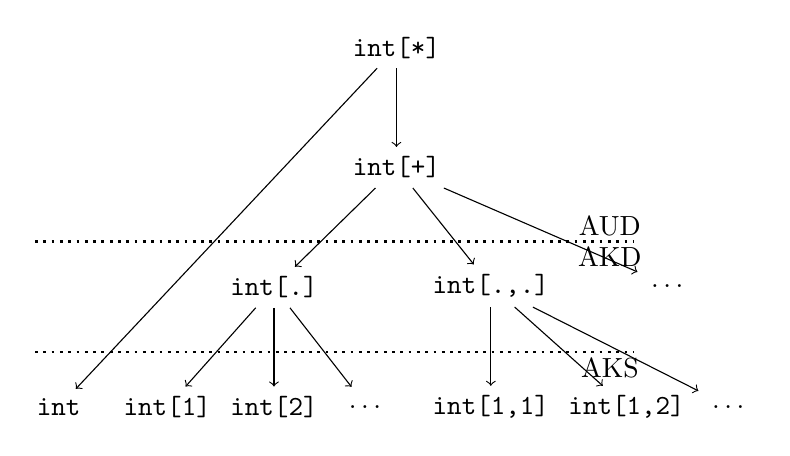
\begin{tikzpicture}
    % AKS scalar
    \node (c) {\texttt{int}};
    % AKS vector
    \node (i1) [right=3mm of c]  {\texttt{int[1]}};
    \node (i2) [right=0mm of i1] {\texttt{int[2]}};
    \node[minimum width=8mm, minimum height=5mm] (in) [right=1mm of i2] {\dots{}};
    % AKS matrix
    \node (i11) [right=3mm of in]  {\texttt{int[1,1]}};
    \node (i12) [right=0mm of i11] {\texttt{int[1,2]}};
    \node[minimum width=8mm, minimum height=5mm] (inn) [right=0.5mm of i12] {\dots{}};
        % AKD
        \node (i)   [above=1cm of i2]  {\texttt{int[.]}};
        \node (ii)  [above=1cm of i11] {\texttt{int[.,.]}};
        \node[minimum width=8mm, minimum height=5mm] (iii) [right=1cm of ii]  {\dots{}};
            % AUD
            \node (plus) [above right=1cm and 2mm of i] {\texttt{int[+]}};
            \node (star) [above=1cm of plus] {\texttt{int[*]}};

    \draw[->] (star) -- (plus);
    \draw[->] (star) -- (c);

    \draw[->] (plus) -- (i);
    \draw[->] (plus) -- (ii);
    \draw[->] (plus) -- (iii);

    \draw[->] (i) -- (i1);
    \draw[->] (i) -- (i2);
    \draw[->] (i) -- (in);

    \draw[->] (ii) -- (i11);
    \draw[->] (ii) -- (i12);
    \draw[->] (ii) -- (inn);

    \draw[dotted, line width=1pt] (-0.3,2.1) -- (7.3,2.1);
    \draw[dotted, line width=1pt] (-0.3,0.7) -- (7.3,0.7);

    \node at (7,2.3) {AUD};
    \node at (7,1.9) {AKD};
    \node at (7,0.5) {AKS};
\end{tikzpicture}
\caption{Hierarchy of integer array types in SaC}
\label{fig:hierarchy}
\end{figure}

\subsection{Domain constraints}

In order to more efficiently check domain constraints imposed by primitive operations on arrays, such as array selection, SaC offers a hybrid approach~\cite{sac-contracts}.
During compilation it inserts checks around primitive functions, such as around the built-in element selection primitive \verb|_sel_VxA_|.
These inserted checks might be statically resolved based on the values, shapes, or ranks of the input.
Depending on whether the arguments are AKV, AKS, or AKD, certain checks can be statically resolved.

Consider this element selection example.
This built-in function expects an array and an index vector with as many elements as the rank of that array.
This index vector must be non-negative and each element must be less than the corresponding shape-element of the array.
It always returns the scalar value at that exact index, and does not allow for the selection of a larger sub-array.
We require two constraints: one to ensure that the length of the selection vector is equal to the rank of the array, and one to check that each value in the selection vector is in bounds of the shape of the array.
Here we can statically resolve the first constraint if the index vector is AKS and the array is only AKD.
Whereas to statically resolve the second constraint we require that the index vector is AKV and the array is AKS.

\subsection{Tensor comprehension}

SaC allows for rank- and shape-invariant programming by means of `tensor comprehensions' \cite{sac-tensor}.
Essentially, tensor comprehensions are a mapping from index vectors to values.
The result of a tensor comprehension is an array, whose shape depends on the range of these index vectors.
For example, we can use tensor comprehensions to increment all values in the variable-rank array \texttt{arr}.
\begin{lstlisting}
inc = { iv -> arr[iv] + 1 };
\end{lstlisting}

\noindent
This index vector \texttt{iv} is a variable-length vector, where the length is based on the usages of \texttt{iv}.
If \texttt{arr} is for example an \texttt{N$\times$M} matrix, \texttt{iv} is a two-element index vector that is repeatedly applied to the increment expression, with values ranging from \texttt{[0,0]} to \texttt{[N-1,M-1]}.

The range of the index vector can usually be inferred automatically from the uses of \texttt{iv}, but may also be defined manually.
For example, we might only want to apply the tensor comprehension to a sub-array of \texttt{arr}.
\begin{lstlisting}
shp = shape(arr) / 2;
inc = { iv -> arr[iv] + 1 | iv < shp };
\end{lstlisting}

\noindent
Here we denote that \texttt{iv} ranges up until and excluding the vector \texttt{shp}.
Because no lower bound is given, it is set to a zero-element vector of the same rank as \texttt{shp}.
Note that the shape of the result \texttt{inc} depends on the range of the index vector \texttt{iv} and not on the array \texttt{arr}, the shape of \texttt{inc} will thus be \texttt{shp} and not \texttt{shape(a)}.

\section{Introducing type patterns}

We introduce type patterns from the perspective of introducing a pattern matching mechanism, as this matches more directly with the way we map them into the pre-existing hybrid type system of SaC.
An alternative way to think about type patterns is to see them as ways to introduce types, through the introduction of variables within type signatures of function definitions.

\subsection{Syntax of type patterns}

We start out with the syntax of type patterns, shown in Figure~\ref{fig:syntax}.

\begin{figure}[hbt]
\begin{verbatim}
<pattern>  ::= <type> '[' <feature> (',' <feature>)* ']'

<feature>  ::= <single>
            |  <multiple>

<single>   ::= '.'
            |  <num>
            |  <id>

<multiple> ::= '*'
            |  '+'
            |  <num> ':' <id>
            |  <id> ':' <id>
\end{verbatim}
\caption{EBNF for type patterns}
\label{fig:syntax}
\end{figure}

\noindent
This syntax extends of the notion of array types from SaC, providing more syntactical flexibility and introducing variables within these types.
Similar to the types in SaC, type patterns consist of an element type followed by a shape specification in square brackets.
The shape specification is a pattern, which consists of a list of `features'.
These features either describe a single rank of the argument, or a larger slice (a sub-vector) of its shape vector.

Single dimensions are captured by the \verb|<single>| rule in Figure~\ref{fig:syntax} and can be denoted by the `\tpdot{}' symbol, a constant number, or a variable name.
A fixed number requires the length of the corresponding rank component to match that very number, whereas the `\texttt{.}' symbol allows for an arbitrary extent.
If instead a variable is being used, the extent found needs to match all other occurrences of that very variable within a given function definition.
For example, consider the type pattern \texttt{int[n,n]}.
It allows for square matrices of arbitrary size $\texttt{n} \times \texttt{n}$ where \texttt{n} is a non-negative integer value.

Rank-polymorphism requires the ability to denote a statically unknown number of ranks.
To cater for this, the proposed type patterns support features that capture slices of a given shape.
These are captured by the \verb|<multiple>| rule in Figure~\ref{fig:syntax}.
We distinguish four cases, depending on the rank of the slice we want to match, and whether we are interested in the slice itself or not.
If we are not interested in the slice itself, we can use one of the symbols `\texttt{+}' and `\texttt{*}'.
They match any slice of at least rank 1 or 0, respectively.

If we are interested in the slice itself, the feature consists of two components separated by a `\texttt{:}' symbol.
The first component relates to the rank of that slice, whereas the second component relates to the slice itself, i.e. the lengths of the corresponding axes.
For the rank component, similar to the single-rank features, we can either use a fixed number or an identifier.
For example, \texttt{int[3:shp]} matches rank 3 arrays only, and matches the entire shape vector against the variable \texttt{shp} that will thus be a three-element vector.
Note here that variables after the `\texttt{:}' symbol, such as \texttt{shp}, denote slices and therefore always represent vectors, even if they match no ranks (empty vector) or individual ranks (singleton vector).
For example, a type pattern \texttt{int[1:n,1:n]}, similar to the \texttt{int[n,n]} example above, matches arbitrary sized square matrices, but \texttt{n} now is a singleton vector rather than a scalar value.

Finally we have the case where the rank of the slice is also a variable, enabling a match of a variable-rank slice of an array shape.
Here, the first component matches against the rank of the slice, and the second component again matches against the slice itself.
For example, the pattern \texttt{int[d:shp]} matches arrays of arbitrary shape, and binds the variable \texttt{d} to the rank of the array, and the variable \texttt{shp} to the shape of the array.

These features can be combined to create complex type patterns.
Consider for example a type pattern \texttt{int[5,n,d:shp]} \texttt{v}.
It matches any shape of at least rank 2, whose extent in the first axis is exactly five, and whose extent in the second axis is \texttt{n}.
Any potentially remaining axes are bound to the vector \texttt{shp}.
These variables (\texttt{n}, \texttt{d}, and \texttt{shp}) can also be used in the function body.
Following are some examples for arguments \texttt{v} and the resulting values of \texttt{n}, \texttt{d}, and \texttt{shp}.

\begin{table}[ht!]
\ttfamily
\begin{tabular}{lllll}\hline
    shape(v)             & 5 & n & d & shp       \\\hline
    \text{}[5,1]         & 5 & 1 & 0 & []        \\
    \text{}[5,1,7]       & 5 & 1 & 1 & [7]       \\
    \text{}[5,0,1,2]     & 5 & 0 & 2 & [1,2]     \\
    \text{}[5,2,1,2,3,4] & 5 & 2 & 4 & [1,2,3,4] \\\hline
\end{tabular}
\end{table}

\noindent
Variable names may be used more than once.
For example, the variable \texttt{n} can be reused in a variable-rank feature \texttt{[5,n,n:shp]}~\texttt{v}.
This pattern matches arrays of at least rank 2 whose extent in the second axis determines the number of ranks that follow.
Some examples of matching shapes are:

\begin{table}[ht!]
\ttfamily
\begin{tabular}{llll}\hline
    shape(v)             & 5 & n & shp       \\\hline
    \text{}[5,0]         & 5 & 0 & []        \\
    \text{}[5,1,0]       & 5 & 1 & [0]       \\
    \text{}[5,1,42]      & 5 & 1 & [42]      \\
    \text{}[5,4,1,2,3,4] & 5 & 4 & [1,2,3,4] \\\hline
\end{tabular}
\end{table}

\noindent
Note that \texttt{d} in the first example, and \texttt{n} in the second example, are equal to the length of \texttt{shp}, which is always the case for such variable-rank patterns.

\subsection{Using type patterns}\label{sec:examples}

Making use of these type patterns, we can extract the shape and the rank of an argument without requiring the use of built-in functions, allowing for simple re-definitions of the functions \texttt{dim} and \texttt{shape}:
\begin{lstlisting}
int                      int[d]
dim(int[d:shp] arr)      shape(int[d:shp] arr)
{                        {
    return d;                return shp;
}                        }
\end{lstlisting}

\noindent
In the example of \texttt{shape} we can see how the type pattern notation allows for an intuitive way to express the relation between the rank of the argument and the shape of the result.

Type patterns also allow us to impose constraints between multiple arguments and return values of a function.
For example, the function signature of shape-polymorphic addition of two floating point arrays can be specified by:
\begin{lstlisting}
float[d:shp]
add(float[d:shp] a, float[d:shp] b)
{
    return { iv -> a[iv] + b[iv] };
}
\end{lstlisting}

\noindent
Here the type patterns in the signature demand both arguments to have the exact same shape.
Additionally it specifies that the shape of the result will also be equal to the shapes of those two inputs.

An example of a more intricate shape relation between argument and result shapes can be seen in a simplified definition of the \texttt{take} function:
\begin{lstlisting}
float[n:shp,m:inner]
take(int[n] shp, float[n:outer,m:inner] arr)
{
    return { iv -> arr[iv] | iv < shp };
}
\end{lstlisting}

\noindent
We see here that the result has the same rank as the second argument, where the first \texttt{n} elements of the result shape are defined through the values of the first argument.
These type patterns demonstrate an interesting case: when looking at the type pattern of argument \texttt{arr} in isolation, we have two features that match against a variable number of ranks captured by the variables \texttt{n} and \texttt{m}.
This is potentially ambiguous.
However, in the given context, we have a uniquely determined constraint for \texttt{n} through the shape of the first argument.

This potential ambiguity is inevitable as soon as we have more than one variable-rank feature within a type pattern.
Fortunately, these cases can be identified and rejected statically, during the translation of type patterns into explicit constraint checking code.

Finally we consider the shape-polymorphic selection function, which uses the \verb|_sel_VxA_| primitive (applied using \texttt{arr[$...$]}) to select a single scalar, or a larger sub-array, from a given array.
This function will serve as our running example throughout the remainder of this paper.
\begin{lstlisting}
int[d:shp]
sel(int[n] idx, int[n:outer,d:shp] arr)
{
    return { iv -> arr[idx ++ iv] | iv < shp };
}
\end{lstlisting}

\noindent
Again, we see here a potential ambiguity between the two variable-rank features of argument \texttt{arr}, captured by the variables \texttt{n} and \texttt{d}.
This ambiguity is resolved through the occurrence of \texttt{n} within the type pattern of the first argument.

\section{Transforming type patterns}

Rather than mapping type patterns and their constraints into some form of dependent types, we instead map them into the existing type system of SaC along with a set of constraints that are inserted into the program.
Revisiting the signature of the selection function from the previous section, we can see that it combines multiple variable-rank features, across multiple argument and return types.
\begin{lstlisting}
int[d:shp]
sel(int[n] idx, int[n:outer,d:shp] arr)
\end{lstlisting}

\noindent
The rank and shape of the result of this function must match \texttt{d} and \texttt{shp} respectively, which are defined by the type pattern of argument \texttt{arr}.
However, that argument has two variable-rank features, captured by the variables \texttt{n} and \texttt{d}.
In this case the value of \texttt{n} is required before the value of \texttt{d} can be computed.
We compute \texttt{n} from the length of the index vector \texttt{idx}, after which we are able to compute the values of \texttt{d} and \texttt{shp}, which finally provides us with the rank and shape of the result.

From this example it becomes clear that the order in which type patterns are resolved matters.
We might need to switch between multiple arguments and features in order to be able to resolve complicated and intertwined dependencies.
To cater for this, we consider type patterns as a constraint resolution problem.
We do so by not only generating the relevant constraints for each feature, but by also including the dependencies that need to be resolved, i.e., the values we need before that constraint can be resolved.

\subsection{Type pattern analysis}\label{sec:atp}

As a first step, we convert type patterns to SaC types.
Looking at the selection example, the index vector is a rank-one array of length \texttt{n}, but because we do not statically know \texttt{n} we have no choice but to convert it to the SaC type \texttt{int[\tpdot]}.
The array argument consists of two variable-rank features, both of which could be empty, thus now the only fitting SaC type is \texttt{int[*]}.
Similarly for the return value, which has a single variable-rank feature of which we have no static knowledge.
Consequently, we need to map the type patterns of the selection function to:
\begin{lstlisting}
int[*]
sel(int[.] idx, int[*] arr)
\end{lstlisting}

\noindent
We formalise this process by means of a recursive transformation function: \texttt{A}nalyse \texttt{T}ype \texttt{P}atterns (\texttt{ATP}).
\begin{gather*}
    \atp{type\_pattern}{\fshp}{\fdim}{\vdim} \\
        = (sac\_type,\ \fshp',\ \fdim',\ \vdim')
\end{gather*}

\noindent
It traverses through the given type pattern, feature by feature, collects information about the features seen so far, until it returns a SaC type along with the information accumulated in three additional parameters:
\begin{enumerate}
    \item \fshp{}: a list of known shape components.
    We denote these by a list of integers enclosed in square brackets, and we start \texttt{ATP} with \texttt{[]}.
    \item \fdim{}: an integer for the minimal number of ranks required, starting with 0.
    \item \vdim{}: a list containing the rank identifiers of variable-rank features (such as \texttt{*} and \texttt{d:shp}).
    We denote these by a list of identifiers enclosed in square brackets, starting with \texttt{[]}.
\end{enumerate}

\noindent
The different cases of \texttt{ATP} directly follow the different options for pattern features.
When the feature is either an individual dot symbol or a variable, we increment \fdim{} to reflect the need for exactly one dimension.
\begin{gather*}
    \atp{type[\tpdot,\rest]}{\fshp}{\fdim}{\vdim} \\
        = \atp{type[\rest]}{\fshp}{\fdim+1}{\vdim}
    \\[2pt]
    \atp{type[id,\rest]}{\fshp}{\fdim}{\vdim} \\
        = \atp{type[\rest]}{\fshp}{\fdim+1}{\vdim}
\end{gather*}
In our rule, we use $\rest$ to denote the (possible empty) remaining features of the type pattern which are needed for the recursive step.

\noindent
Similarly for integers \tpnum{}, but since that value describes the extent of a rank, we also add that integer to the list of known shapes.
This is the only case where the number of known shapes is changed.
\begin{gather*}
    \atp{type[\tpnum,\rest]}{\fshp}{\fdim}{\vdim} \\
        = \atp{type[\rest]}{\fshp \text{ ++ } [\tpnum]}{\fdim+1}{\vdim}
\end{gather*}

\noindent
If instead we match on a shape-component with some constant non-negative integer rank \texttt{n}, that feature describes the shape-component of the following \texttt{n} ranks, so we increase the number of known ranks by that amount.
We ignore the $shp$ identifier because it has no impact on the resulting type.
\begin{gather*}
    \atp{type[\tpnumshp{shp},\rest]}{\fshp}{\fdim}{\vdim} \\
        = \atp{type[\rest]}{\fshp}{\fdim+\tpnum}{\vdim}
\end{gather*}

\noindent
When this rank is instead an identifier $d$, we append that identifier to the list of variable ranks.
We do not increase the number of known ranks, because $d$ is potentially zero.
\begin{gather*}
    \atp{type[\tpidshp{d}{shp},\rest]}{\fshp}{\fdim}{\vdim} \\
        = \atp{type[\rest]}{\fshp}{\fdim}{\vdim \text{ ++ } [d]}
\end{gather*}

\noindent
Finally, when we encounter a \tpstar{} we simply add it to the list of variable ranks as well.
We have a similar case if we encounter a \tpplus{}, but since it describes a shape with a non-zero rank, we also increment the number of known ranks.
\begin{gather*}
    \atp{type[\tpstar,\rest]}{\fshp}{\fdim}{\vdim} \\
        = \atp{type[\rest]}{\fshp}{\fdim}{\vdim \text{ ++ } [\tpstar{}]}
    \\[2pt]
    \atp{type[\tpplus,\rest]}{\fshp}{\fdim}{\vdim} \\
        = \atp{type[\rest]}{\fshp}{\fdim+1}{\vdim \text{ ++ } [\tpstar{}]}
\end{gather*}

\noindent
Once the function is applied to all features,
the resulting SaC type can be determined:
\begin{gather*}
    \atp{type[]}{\fshp}{\fdim}{\vdim} = (T,\ \fshp,\ \fdim,\ \vdim) \\
        \text{where} \\
        T = \begin{cases}
            type\texttt{[*]}
                &\text{if } |\vdim| > 0
                \text{ and } \fdim =\hspace{0.6pt} 0 \\
            type\texttt{[+]}
                &\text{if } |\vdim| > 0
                \text{ and } \fdim > 0 \\
            type[\tpdot_{_1}, ..., \tpdot_{_n}]
                &\text{if } |\vdim| =\hspace{0.6pt} 0
                \text{ and } \fdim = n > |\fshp| \\
            type[\fshp]
                &\text{if } |\vdim| =\hspace{0.6pt} 0
                \text{ and } \fdim = |\fshp|
        \end{cases}
\end{gather*}

\noindent
If \vdim{} is not empty, the type has an unknown rank that is at least of length \fdim{}.
Otherwise, we statically know that the rank of the array is equal to \fdim{}.
Furthermore, if the number of known shapes and ranks are equal, the type pattern only contains constant rank sizes, such as \texttt{int[5,3,7]}, and thus the shape is statically known.

As an example we consider a type pattern \texttt{int[5,n,d:shp]}.
Applying \texttt{ATP} to it gives:
\begin{align*}
    &\atp{\texttt{int[\textbf{5},n,d:shp]}}{0}{0}{[]} \\
    &= \atp{\texttt{int[\textbf{n},d:shp]}}{1}{1}{[]} \\
    &= \atp{\texttt{int[\textbf{d:shp}]}}{1}{2}{[]} \\
    &= \atp{\texttt{int[]}}{1}{2}{[d]} \\
    &= (\texttt{int[+]},\ 1,\ 2,\ [d])
\end{align*}

\noindent
This results in a known rank of at least two, but because there are also variable ranks the resulting SaC type is \texttt{int[+]}.

\subsection{Constraint generation}\label{sec:gtc}

The next step is to aggregate all possible constraints that result from type patterns.
We use a similar approach as in the previous section, recursing through the features of a type pattern and collecting information of the resulting constraints.
The basic idea is to accumulate an environment of constraints for all variables.

This constraint aggregation poses two particular challenges.
Firstly, we may find constraints for a single pattern variable within more than one type pattern of a function signature.
This implies that we cannot look at single type patterns in isolation.
We resolve this issue by collecting an environment of constraints and by passing this environment from one type pattern within a function signature to the next.
Secondly, we can have dependencies between constraints:
As soon as there is a variable-rank feature combined with any other feature, any resolution process can no longer be done in arbitrary order. We record such dependencies as we generate the environment of constraints.

We denote our constraint environment by entries of the form:
\begin{align*}
    var \mapsto [\langle{}expr_1,\ deps_1\rangle,\ \dots,\ \langle{}expr_n,\ deps_n\rangle]
\end{align*}

\noindent
where $var$ refers to any variable name occurring in a given function signature, be it in a type pattern or an argument name itself.
Each tuple $\langle{} expr_i,\ deps_i \rangle$ represents a SaC expression $expr_i$ that constitutes the constraint for $var$.
I.e. at runtime, the value of $var$ needs to be identical to the value of that expression, and $deps_i$ contains the set of variables that stem from variable-rank features and are referred to within $expr_i$.

For example, for a function argument \texttt{int[d,d:shp]} \texttt{v}, we want to infer the following two environment entries:
\begin{align*}
    \mathbf{\{}\
        d   \mapsto [&\langle\texttt{shape}(v)[0],\ \emptyset\rangle, \\
                     &\langle\texttt{dim}(v)-1,\ \emptyset\rangle] \\
        shp \mapsto [&\langle\texttt{take}(d,\ \texttt{drop}(1,\ \texttt{shape}(v))),\ \{d\}\rangle]
    \ \mathbf{\}}
\end{align*}

\noindent
For inferring such constraint environments, we define a function: \texttt{G}enerate \texttt{T}ype \texttt{C}onstraints (\texttt{GTC}).
\begin{gather*}
    \texttt{GTC}(type\_pattern,\, \cdim,\, \deps,\, \cenv) = \cenv'
\end{gather*}

\noindent
It is being successively applied to all type pattern of any given type signature and accumulates a constraint environment \cenv{} for the entire signature
while doing so.
In addition to the current type pattern and the constraint environment to be generated,
it uses two further parameters when
being applied to each individual type pattern within a function signature.
These parameters are:
\begin{enumerate}
    \item \cdim{}: the current position in the shape vector of the argument, starting with 0.
    \item \deps{}: a set of variable-rank identifiers encountered so far.
\end{enumerate}

\noindent
Following are the recursive cases of the \texttt{GTC} function.
In the case that we encounter a dot, we only need to increment the current position in the shape.
Because in this case we do not care about the result, no constraints are added to the environment.
\begin{gather*}
    \gtc{type[\tpdot,\rest]}{\cdim}{\deps}{\cenv} \\
        = \gtc{type[\rest]}{\cdim+1}{\deps}{\cenv}
\end{gather*}

\noindent
For constant integers \tpnum{} we similarly increment the current shape position.
However now we also add a constraint to the environment of the argument with the current dependencies.
This constraint gets the extent of the current rank from the current shape position, and checks that it is equal to \texttt{n}.
We write $\cenv[var \mapsto \langle{}expr,\ deps\rangle{}]$ to denote that the environment \cenv{} is extended with a new entry $\langle{}expr,\ deps\rangle{}$ for the constraints list of $var$.

{
\topskip0pt
\setlength\abovedisplayskip{0pt}
\begin{gather*}
    \gtc{type[\tpnum,\rest]}{\cdim}{\deps}{\cenv} \\
        = \gtc{type[\rest]}{\cdim+1}{\deps}{ \\ \cenv
            \envmap{v}{\deps}{\tpnum == \texttt{shape}(v)[\cdim]}}
\end{gather*}
}

\noindent
We have a similar case if we encounter an identifier $id$.
However we now add a constraint to the environment for $id$ instead.
\begin{gather*}
    \gtc{type[id,\rest]}{\cdim}{\deps}{\cenv} \\
        = \gtc{type[\rest]}{\cdim+1}{\deps}{ \\ \cenv
            \envmap{id}{\deps}{\texttt{shape}(v)[\cdim]}}
\end{gather*}

\noindent
In the case of a shape of fixed length \tpnum{}, we instead increase the current shape position by this fixed amount.
We also add a constraint for the shape identifier $shp$ with the current dependencies.
This constraint drops the first \cdim{} dimensions from the shape, and then takes the following \tpnum{} elements to get the $shp$ vector.
\begin{gather*}
    \gtc{type[\tpnumshp{shp},\rest]}{\cdim}{\deps}{\cenv} \\
        = \gtc{type[\rest]}{\cdim+\tpnum}{\deps}{ \\ \cenv
            \envmap{shp}{\deps}{\texttt{take}(\tpnum,\ \texttt{drop}(\cdim,\ \texttt{shape}(v)))}}
\end{gather*}

\noindent
For variable-rank features we have a somewhat similar case.
Instead of increasing the current position by a fixed value, we increase it by $d$.
Since $d$ is a variable-rank identifier we add it to the accumulated dependencies.
We also have a similar constraint for $shp$, where instead we take $d$ elements.
Here again because $d$ is a variable-rank identifier, we add it to the dependencies of this constraint.

Additionally a constraint for $d$ itself is required.
We get this constraint from the dimensionality of $v$, by subtracting from it the minimal rank of $v$ found by \texttt{ATP} ($v.\fdim$) as well as the variable-rank identifiers found by \texttt{ATP} ($v.\vdim$), excluding $d$.
We compute this as $\texttt{dim}(v) - v.\fdim - \texttt{sum}(v.\vdim) + d$, which we hereafter shorten to $\texttt{dimcalc}(v,\ d)$.
\begin{gather*}
    \gtc{type[\tpidshp{d}{shp},\rest]}{\cdim}{\deps}{\cenv} \\
        = \gtc{type[\rest]}{\cdim+d}{\deps \cap \{d\}}{ \\ \cenv
            \envmap{d}{v.\vdim \setminus \{d\}}{\texttt{dimcalc}(v,\ d)} \\
            \envmap{shp}{\deps \cap \{d\}}{\texttt{take}(d,\ \texttt{drop}(\cdim,\ \texttt{shape}(v)))}}
\end{gather*}

\noindent
Finally we have the cases for \tpstar{} and \tpplus{}.
In the case of \tpstar{} there is nothing more to do, and we continue with the next feature.
If instead we encounter a \tpplus{}, we increment the current shape position before continuing.
\begin{gather*}
    \gtc{type[\tpstar,\rest]}{\cdim}{\deps}{\cenv} \\
        = \gtc{type[\rest]}{\cdim}{\deps}{\cenv}
    \\[2pt]
    \gtc{type[\tpplus,\rest]}{\cdim}{\deps}{\cenv} \\
        = \gtc{type[\rest]}{\cdim+1}{\deps}{\cenv}
\end{gather*}

\noindent
In certain scenarios it is possible that these generated constraints cause an out-of-bounds selection.
Consider a variable-rank feature where the input is expected to be of at least rank three.
Since \texttt{ATP} will convert this type pattern to the type \texttt{int[+]}, a rank one or two input will not be seen as a type error by the type-checker.
As a result, such a lower rank input will instead cause an out-of-bounds exception in the generated code when trying to construct features that expect an input of at least rank three.
To avoid generating erroneous code, we additionally add a constraint to ensure that the rank of the argument is large enough to fit the given type pattern.

\noindent
This is done by comparing the rank of the argument $v$ to the minimal rank that was found by \texttt{ATP} ($v.\fdim$).
If there are no variable ranks we check whether the rank is exactly equal to the number of known ranks (1), otherwise we check whether the argument has at least that many ranks (2).

This results in the following base case:
\begin{gather*}
    \gtc{type[]}{\cdim}{\deps}{\cenv} \\
        = \begin{cases}
            \cenv\envmap{v}{\emptyset}{\texttt{dim}(v) == v.\fdim}
                &\text{if } \vdim = \emptyset
                \hspace{10pt}(1) \\
            \cenv\envmap{v}{\emptyset}{\texttt{dim}(v) >= v.\fdim}
                &\text{otherwise}
                \hspace{14.5pt}(2)
        \end{cases}
\end{gather*}

\noindent
Consider again the example \texttt{int[5,n,d:shp]} with a mapping \cenv{} that might have been populated by type patterns of previous arguments.
In each step \texttt{GTC} resolves a single feature from the type pattern.
This results in an updated environment with a constraint for each identifier, along with a constraint that checks the rank of the argument.
{\allowdisplaybreaks
\begin{align*}
    &\gtc{\texttt{int[\textbf{5},n,d:shp]}}{0}{\emptyset}{\cenv} \\
    &= \gtc{\texttt{int[\textbf{n},d:shp]}}{1}{\emptyset}{
        \\ &\hspace{3em} \cenv
        \envmap{v}{\emptyset}{5 == \texttt{shape}(v)[0]}
    } \\
    &= \gtc{\texttt{int[\textbf{d:shp}]}}{2}{\emptyset}{
        \\ &\hspace{3em} \cenv
        \envmap{v}{\emptyset}{5 == \texttt{shape}(v)[0]}
        \\ &\hspace{3.6em}
        \envmap{n}{\emptyset}{\texttt{shape}(v)[1]}
    } \\
    &= \gtc{\texttt{int[]}}{2+d}{\{d\}}{
        \\ &\hspace{3em} \cenv
        \envmap{v}{\emptyset}{5 == \texttt{shape}(v)[0]}
        \\ &\hspace{3.6em}
        \envmap{n}{\emptyset}{\texttt{shape}(v)[1]}
        \\ &\hspace{3.6em}
        \envmap{d}{\emptyset}{\texttt{dimcalc}(v,\ d)}
        \\ &\hspace{3.6em}
        \envmap{shp}{\{d\}}{\texttt{take}(d,\ \texttt{drop}(2,\ \texttt{shape}(v)))}
    } \\
    &= \cenv
        \envmap{v}{\emptyset}{5 == \texttt{shape}(v)[0]}
        \\ &\hspace{1.8em}
        \envmap{n}{\emptyset}{\texttt{shape}(v)[1]}
        \\ &\hspace{1.8em}
        \envmap{d}{\emptyset}{\texttt{dimcalc}(v,\ d)}
        \\ &\hspace{1.8em}
        \envmap{shp}{\{d\}}{\texttt{take}(d,\ \texttt{drop}(2,\ \texttt{shape}(v)))}
        \\ &\hspace{1.8em}
        \envmap{v}{\emptyset}{\texttt{dim}(v) >= 2}
\end{align*}}

\newcommand{\defined}{\texttt{defined}}
\renewcommand{\exists}{\texttt{exists}}

\section{Constraint resolution}

We take a partial evaluation approach based on the idea of symbiotic expressions~\cite{sac-symbiotic}.
Symbiotic expressions provide a method for algebraic simplification, based on expressions inserted into the code.
We take a similar approach, by inserting the generated constraints into the program.
Similarly to symbiotic expressions, the insertion of this code can potentially lead to further optimisation.
Unlike symbiotic expressions, we propose that the inserted code is not necessarily removed after optimisation, in order to allow for run-time errors for constraints that could not statically be resolved.

\subsection{Resolution algorithm}\label{sec:resoltion}

Now that we have the necessary constraints for all arguments and features of a function signature, the next step is to transform each of those constraints to either a variable assignment, or to a boolean check expression.
As discussed previously, the order in which the code for these constraints is inserted into the program is important.

\noindent
We use the dependencies found by \texttt{GTC} to derive the correct ordering.
Following is the description of an algorithm that uses the dependencies to generate an ordered list of assign statements and check expressions, ensuring that the dependencies of those constraints are resolved in the correct order.

We require two additional sets for this algorithm:
\begin{enumerate}
    \item \defined{}: a set which contains all identifiers that have thus far been defined.
    Initially, these are only the arguments themselves.
    \item \exists{}: a set which contains all identifiers that have remaining constraints.
    These are initially all identifiers that occur in the type patterns of the function signature.
\end{enumerate}

\noindent
This results in two ordered lists for the generated assignments and checks.
These two lists will be inserted into the code as described in section~\ref{sec:generation}.
The algorithm is repeated until no more code can be generated.
At that point either every constraint has been resolved, or there are multiple constraints that cannot be resolved because they depend on each other in some way, in which case we raise an error and print the constraints that could not be resolved.

\begin{figure}[hbt]
\begin{lstlisting}[language=pseudocode]
changed = true;

while changed:
  changed = false

  for id in exists:
    all_dependencies_resolved = true

    constraints = env[id]
    for entry in constraints:
      deps, expr = entry
      if union(deps, defined) is not empty:
        all_dependencies_resolved = false
        continue

      if id is not in defined:
        assignments += create_assign(id, expr)
        defined += {id}
      else:
        checks += create_check(id, expr)

      env[id] -= {entry}
      changed = true

    if all_dependencies_resolved:
      exists -= {id}
\end{lstlisting}
\caption{Pseudo-code for the resolution algorithm}
\label{fig:resolution-algorithm}
\end{figure}

The algorithm described in Fig.~\ref{fig:resolution-algorithm} iterates over all identifiers in the \exists{} set, which are the identifiers that have remaining constraints.
It then iterates over the remaining constraints of those identifiers.
If a constraint has dependencies that are not yet defined, then this constraint still has unresolved dependencies and is skipped.
Otherwise there is a case distinction depending on whether the identifier itself has a definition yet.
If not, an assignment to this identifier is generated from the value of the constraint and the identifier is added to the \defined{} set.
Otherwise there already exists such a definition, and instead a check is generated to ensure that this definition is equal to the value of the constraint.

Finally the entry is removed from the environment and we continue with the next constraint.
After no more changes occur, if \exists{} is empty all constraints were able to be resolved, otherwise we have an ambiguous case and \exists{} contains the remaining constraints that could not be resolved due to circular dependencies.

To illustrate such an ambiguous case we take another look at the selection function example.
If we consider the array argument \texttt{int[n:outer,d:shp]} in isolation, we would receive the following environment \cenv{} from \texttt{GTC}:
\begin{align*}
    \mathbf{\{}\
        \underline{n} \mapsto [&\langle\texttt{dimcalc}(arr,\ n),\ \{\underline{d}\}\rangle] \\
        outer         \mapsto [&\langle\texttt{take}(n,\ \texttt{drop}(0,\ \texttt{shape}(arr))),\ \{n\}\rangle] \\
        \underline{d} \mapsto [&\langle\texttt{dimcalc}(arr,\ d),\ \{\underline{n}\}\rangle] \\
        shp           \mapsto [&\langle\texttt{take}(d,\ \texttt{drop}(n,\ \texttt{shape}(arr))),\ \{n,d\}\rangle]
    \ \mathbf{\}}
\end{align*}

\noindent
Here we immediately see an example of an ambiguous case that cannot be resolved by our algorithm, as \texttt{n} depends on \texttt{d} and vice versa.
Already in the first iteration of the algorithm there is nothing that can be done, since each constraint has remaining dependencies.
However if we include the index vector argument \texttt{int[n]}, a new entry is added in the environment for identifier \texttt{n}:
\begin{align*}
    \mathbf{\{}\
        n     \mapsto [&\langle\texttt{dimcalc}(arr,\ n),\ \{d\}\rangle, \\
            &\underline{\langle\texttt{shape}(idx)[0],\ \emptyset\rangle}] \\
        outer \mapsto [&\langle\texttt{take}(n,\ \texttt{drop}(0,\ \texttt{shape}(arr))),\ \{n\}\rangle] \\
        d     \mapsto [&\langle\texttt{dimcalc}(arr,\ d),\ \{n\}\rangle] \\
        shp   \mapsto [&\langle\texttt{take}(d,\ \texttt{drop}(n,\ \texttt{shape}(arr))),\ \{n,d\}\rangle]
    \ \mathbf{\}}
\end{align*}

\noindent
In this case the algorithm is able to generate an assignment for this new constraint of \texttt{n}, because it has no dependencies.
This results in \texttt{n} being added to the \defined{} set.
Now that \texttt{n} is defined, the constraint for \texttt{d} can be resolved and an assignment to \texttt{d} is generated.
Afterwards, the identifiers \texttt{n} and \texttt{d} are both defined and all remaining constraints can be resolved: an assignment is generated for \texttt{outer} and \texttt{shp}, and because \texttt{n} already exists a check is generated for the remaining constraint of \texttt{n}.

\subsection{Code generation}\label{sec:generation}

At this point these ordered lists of generated assignments and checks can be inserted into the program.
Special care needs to be taken to ensure that the generated code is inserted at the most optimal location in the program.

To provide the compiler with as much static information as possible, the generated assignments and checks should preferably be inserted around the call site of the corresponding function, where typically more information about the rank, shape, or values of the arguments is statically available.
This makes it more likely that the checks can statically be resolved, allowing for more type errors at compile time and reducing overhead at run-time.
However a static dispatch is not always possible, such as for overloaded functions.
In this case we have no choice but to insert the generated code into the function body instead.

To cater for both cases with a single implementation, we rely on the inlining capabilities of the compiler.
Inlining ensures that if a call site of a function has been statically dispatched, that call site is replaced by the body of the corresponding function, which typically allows for better optimisation.

To illustrate how the code generation is implemented we continue with the selection function as our running example:
\begin{lstlisting}
int[d:shp]
sel(int[n] idx, int[n:outer,d:shp] arr)
{
    return { iv -> arr[idx ++ iv] | iv < shp };
}
\end{lstlisting}

\noindent
In order to make use of the inlining capabilities of the compiler, we wrap this implementation function into a stub that we always allow to be inlined.
This stub first checks the constraints of the given arguments with a new inline function \texttt{sel\_pre}, and then applies the original function definition \texttt{sel\_impl}.
This replacement ensures that all applications of \texttt{sel} now point to this new function definition containing the corresponding checks, making it possible to execute this compiler step early in the compilation process, before function calls have been dispatched.
Now if an application of \texttt{sel} is able to be dispatched, the generated checks can be inlined to the call site of this function application.
\begin{lstlisting}
inline int[*]
sel(int[.] idx, int[*] arr)
{
    pred = sel_pre(idx, arr);
    result = sel_impl(idx, arr);
    return result;
}
\end{lstlisting}

\noindent
Note that the arguments themselves no longer contain type patterns and are now SaC types, as these were transformed by \texttt{ATP} in section \ref{sec:atp} in order to make these function signatures compatible with the type checker.

Similarly to \cite{sac-contracts}, we need to ensure that the compiler does not optimise away the generated checks.
To achieve this we define a new primitive function: \texttt{guard}, that acts as a barrier for optimisation and code re-writes.
This function expects \texttt{n} arbitrary values, \texttt{n} corresponding types, and a boolean predicate.
Each type at index $i$ is the type of the corresponding value at index $i$ as it has been defined by the function signature.
The types of the result values of these guards are then based on these type arguments, instead of the actual types of these arguments.
We require this to avoid premature optimisation resulting from a specialisation of the arguments.
Then if the predicate is true this guard function behaves as an identity function on these \texttt{n} arguments, otherwise an error is raised and the program aborts.
This behaviour can occur at run-time, but also at compile-time, allowing the compiler to optimise away checks that are statically known to be true.

We surround the application of \texttt{sel\_impl} with guards on the input values and the result value, that rely on the predicate returned by \texttt{sel\_pre}.
This avoids premature optimisations based on either the input values or output type of \texttt{sel\_impl}.
\begin{lstlisting}
inline int[*]
sel(int[.] idx, int[*] arr)
{
    pred = sel_pre(idx, arr);
    idx, arr = guard(idx, arr,
                     int[.], int[*], pred);
    result = sel_impl(idx, arr);
    result = guard(result, int[*], pred);
    return result;
}
\end{lstlisting}

\noindent
Since the implementation function might make use of the variables defined in the type patterns of its arguments, we prepend the generated assignment to the original function body.
This allows the variable \texttt{shp} from the selection example to be used directly in the body of that function.
\begin{lstlisting}[escapechar=@]
int[*]
sel_impl(int[.] idx, int[*] arr)
{
    n = shape(idx)[0];
    outer = take(n, shape(arr));
    d = dim(arr) - n;
    @\underline{shp}@ = take(d, drop(n, shape(arr)));

    return { iv -> arr[idx ++ iv] | iv < @\underline{shp}@ };
}
\end{lstlisting}

\noindent
As opposed to the \texttt{sel} stub, this implementation function is not always inlined.
We only inline this implementation function if the developer marked the original function as inline, which avoids us from inlining a function that the developer did not intend to.

The body of the check function \texttt{sel\_pre} contains the generated assignments, followed by the generated checks.
If all checks succeed true is returned, otherwise we abort the program with a descriptive error message.
In order to comply with the type checker, these aborts are of the same type as \texttt{pred}.
They are weaved into the program using if-expressions, which makes it easy to insert additional checks and makes for a simple and readable implementation.
\begin{lstlisting}
inline bool
sel_pre(int[.] idx, int[*] arr)
{
    n = shape(idx)[0];
    outer = take(n, shape(arr));
    d = dim(arr) - n;
    shp = take(d, drop(n, shape(arr)));

    pred = true;
    pred = n == dim(arr) - d ? pred
        : abort("Type pattern error ...");
    return pred;
}
\end{lstlisting}

\noindent
A drawback of pulling the generated assignments and checks out of the original function definition and moving them to separate functions, is that we require two instances of the assignments to the features of type patterns, once in the check in \texttt{sel\_pre}, and once in the implementation function \texttt{sel\_impl}.
This drawback is mitigated by the fact that performance-critical code is often inlined, in which case common sub-expression elimination can be applied to remove these duplicate definitions.
Additionally, these functions might insert assignments for features that are not used in the function body, such as the variable \texttt{outer} from the example.
This issue is easily resolved by applying dead code removal.

\subsection{Type patterns for return types}

Thus far we have only considered the code generation for type patterns of arguments, but as we have seen in our running selection example, it is also possible to define type patterns on return types.
\begin{lstlisting}
int[d:shp]
sel(int[n] idx, int[n:outer,d:shp] arr)
{
    return { iv -> arr[idx ++ iv] | iv < shp };
}
\end{lstlisting}

\noindent
To support this we extend the definition of \texttt{sel} that was given in section~\ref{sec:generation}.
As opposed to the pre-check function, we insert a post-check function after the result has been computed and check whether that result adheres to the given type pattern constraints.
As before, we include a guard to avoid these checks from being prematurely optimised away.
\begin{lstlisting}[escapechar=@]
inline int[*]
sel(int[.] idx, int[*] arr)
{
    pred = sel_pre(idx, arr);
    idx, arr = guard(idx, arr,
                     int[.], int[*], pred);
    result = sel_impl(idx, arr);
    result = guard(result, int[*], pred);
    @\underline{pred'}@ = sel_post(idx, arr, result);
    result = guard(result, int[*], @\underline{pred'}@);
    return result;
}
\end{lstlisting}

\noindent
The post-check function behaves similarly to the pre-check function, however it additionally expects the results of the implementation and checks whether those values adhere to the constraints imposed by their type patterns.
In the case of our selection example, this means that we insert checks to compare the rank and shape of the result against the features \texttt{d} and \texttt{shp} respectively.
\begin{lstlisting}[escapechar=@]
inline bool
sel_post(int[.] idx, int[*] arr, int[*] @\underline{result}@)
{
    n = shape(idx)[0];
    outer = take(n, shape(arr));
    d = dim(arr) - n;
    shp = take(d, drop(n, shape(arr)));

    pred = true;
    pred = d == dim(@\underline{result}@) ? pred
        : abort("Type pattern error ...");
    pred = all(shp == shape(@\underline{result}@)) ? pred
        : abort("Type pattern error ...");
    return pred;
}
\end{lstlisting}

\noindent
The addition of return-type constraints requires us to determine whether a feature occurring in a return type should be converted to an assignment or to a check within the post-check function.
In the case of our selection example, the features \texttt{d} and \texttt{shp} of the return type are both already defined by the argument \texttt{arr}, thus in the post-check function we generate two expressions to check whether the rank and shape of the result match \texttt{d} and \texttt{shp} respectively.

However, consider a case where the return type is \texttt{int[m,m]}.
Because \texttt{m} has not been defined in any of the arguments of the function signature, we are required to first generate an assignment to \texttt{m} instead.
Namely, we first need to generate \texttt{m = shape(result)[0]}.
This variable can then be used for the comparison of the second feature, \texttt{m == shape(result)[1]}.
This distinction allows us to define constraints within a single return type, or between multiple return types, that are not dependent on the arguments.

In order to be able to make this distinction, it is no longer sufficient to only keep track of a single list of assignments and checks.
Instead, in the algorithm described in section~\ref{sec:resoltion} we make a distinction between assignments and checks that are generated for type patterns of arguments, and assignments and checks that are generated for type patterns of return types.
All that is required is a case distinction, based on whether the constraint originates from the feature of an argument, or the feature of a return type.
For the sake of brevity we do not discuss the exact implementation.

\section{Arbitrary constraints}

Type patterns alone are not yet sufficient for generating arbitrarily complex constraints on arguments and return values.
To preserve the benefits provided by keeping these dependencies contained to the function signature, we extend the syntax of functions by allowing them to contain any number of arbitrary expressions that operate on arguments, or on features of type patterns.
These conditions can be any built-in or user-defined boolean expression without side-effects.

In the case of the selection function, we can include two additional conditions to check whether the index vector is non-negative, and that each index in the index vector is less than the corresponding element in the shape of the array.
Ensuring that the index is always in bounds.
\begin{lstlisting}
int[d:shp]
sel(int[n] idx, int[n:outer,d:shp] a)
    | all(0 <= idx), all(idx < outer)
{
    return { iv -> a[idx ++ iv] | iv < shp };
}
\end{lstlisting}

\noindent
Because of the way we interleave constraints into the pre- and post-check functions, inserting such checks into the program requires little additional effort.
The only significant work that remains is to decide for each condition whether it is a pre-condition, or a post-condition.
If all variables that appear in a condition are defined by arguments or type patterns of arguments in a function signature, then we add a case to the pre-check function for this condition.
Otherwise, if at least one variable occurring in the condition is only defined in the type patterns of the return values, we add that condition to the post-check function instead.

As with the other checks, the condition will be inserted into the code with an if-expression and an as precise as possible error message that describes which condition failed.
The pre-check function, as previously defined in section \ref{sec:generation}, can now easily be extended to include these two new conditions:
\begin{lstlisting}[escapechar=@]
inline bool
sel_pre(int[.] idx, int[*] arr)
{
    n = shape(idx)[0];
    outer = take(n, shape(arr));
    d = dim(arr) - n;
    shp = take(d, drop(n, shape(arr)));

    pred = true;
    pred = n == dim(arr) - d ? pred
        : abort("Type pattern error ...");
    pred = @\underline{all(0 <= idx)}@ ? pred
        : abort("Type pattern error ...");
    pred = @\underline{all(idx < outer)}@ ? pred
        : abort("Type pattern error ...");
    return pred;
}
\end{lstlisting}

\noindent
We similarly extend the post-check function, for any remaining conditions that operate on features of return types.
In the case of our selection example, the post-check function remains unchanged.
Inserting the conditions into these functions allows them to potentially be statically analysed, just as the checks generated by the type patterns.
Whilst we are not able to generate an error message as precise as for type patterns, we are still able to tell the programmer which of the given conditions failed.

With the addition of these feature, our type patterns now provide a complete implementation that is strong enough to support arbitrarily complex conditions, allowing constraints on arguments and return values to be defined entirely in the function signature.
Fully separating such domain constraints from the actual logic of these functions.

\section{Case study}

In section~\ref{sec:examples} we have seen an implementation of the \texttt{take} function, which is used in practice in many array programs.
Applications of this function are prone to out-of-bounds errors: the shape vector argument can have too many elements, or one of its elements can be greater than the corresponding extent in the array argument.
Following is an example of this first case, where the array argument is one-dimensional but a two-element shape argument is provided.
\begin{lstlisting}
arr = genarray ([10], 0f);
res = take ([7,9], arr);
\end{lstlisting}

\noindent
Without the use of type patterns, this invalid application of \texttt{take} produces the following compile time error:
\begin{lstlisting}[language=console]
argument #1 should not exceed the shape of
argument #2 of "_drop_SxV_"; types found:
int{2} and int[1]
\end{lstlisting}

\noindent
This error may come at a surprise as our program does not even make direct use of \verb|_drop_SxV_|.
To find out where this comes from, users can enable a stack trace. For our example, this yields:
\begin{lstlisting}[language=console,escapechar=@]
./example.sac:6: error:
   -- in Array::sel( int[2], float[.])
@\vspace{-7pt}@
./example.sac:12: error:
   -- in _MAIN::take( int[2]{7,9}, float[.])
@\vspace{-7pt}@
./example.sac:18: error:
   -- in _MAIN::foo( float[.])
\end{lstlisting}

\noindent
In this case, we can see that the failing application of \verb|_drop_SxV_| stems from a call to the selection function
in the standard library (here: \verb|Array|) which in turn was called by our version of \verb|take|. However,
it is not immediately clear that an erroneous call of \verb|take| is the culprit, as we see the entire stack trace.
In particular when dealing with long call sequences, a manual check where the unwanted function call happens can become very tedious.

In contrast, the type pattern described in this paper enable the compiler to directly point to the erroneous call.
With type patterns, we get the following pre-condition compile time error:
\begin{lstlisting}[language=console]
Type pattern error in application of take:
dimensionality of argument `arr' is too small,
could not assign a non-negative value to `m'
in `m:inner'
\end{lstlisting}

\noindent
Similarly, type patterns also improve error messages from function implementations that do not meet the co-domain constraints, even if the domain constraints are met.
For example, let us assume a problem within the definition of take, where the upper bound incorrectly uses a $\leq$ instead of $<$, i.e., we have:
\begin{lstlisting}
return { iv -> arr[iv] | iv <= shp };
\end{lstlisting}

\noindent
Furthermore, let us assume we now call \verb|take([10], arr)|.
Without type patterns, we get an error from the out of bounds selection:
\begin{lstlisting}[language=console]
Scalar constraint `SACp_eat_43 (10) <
SACp_emal_7118__uprf_2476 (10)' violated
\end{lstlisting}

\noindent
If we add type patterns to the definition of \texttt{take} we instead get a more descriptive post-condition error message, which makes it clear that there is a mistake in the definition of \texttt{take}:
\begin{lstlisting}[language=console]
Type pattern error in definition of take: the
found value of `shp' in `n:shp' of the return
value is not equal to the value of argument `shp'
\end{lstlisting}

\noindent
We even obtain this error for examples such as \verb|take([8], arr)| where this bug goes unnoticed in the variant without type patterns.

\newcommand{\slicepatterns}{\url{https://blog.rust-lang.org/2018/05/10/Rust-1.26.html\#basic-slice-patterns}}
\newcommand{\subslicepatterns}{\url{https://blog.rust-lang.org/2020/03/12/Rust-1.42.html\#subslice-patterns}}
\newcommand{\listpatterns}{\url{https://learn.microsoft.com/dotnet/csharp/language-reference/operators/patterns\#list-patterns}}

\section{Related work}

\textbf{Dependent types.}
Previous work has investigated the effectiveness of dependent types in practise, in languages such as Agda, Idris, Cayenne, and Coq~\cite{agda, idris, cayenne, coq}.
Such dependently types languages require that a given program can be fully analysed statically.
This requirement can lead to undecidability and non-terminating type checking, especially in the context of rank-polymorphic programs.
This requirement of static analysis is often not feasible in practise, for example when reading input from a file, or for other I/O operations.
These cases would require explicit assertions on program inputs, or might require additional proofs to be given by the developer to aid the type system with proving static correctness.
This undermines our quest for readability and programming productivity.
Instead, we implement a hybrid approach that does not enforce that all constraints can be resolved statically, by instead allowing some constraints to be checked dynamically at run-time.
By doing so we lose the guarantee that any program that can be compiled is also total.
But we avoid undecidability and non-termination by deferring the constraints that could not be resolved statically to run-time, where they can always be checked dynamically.

% Qube
Another approach based on dependent types is to instead encode constraints as first-order formulas, and verify them in collaboration with a theorem prover.
This is the method applied by Qube~\cite{qube}, by using the Yices theorem prover~\cite{yices}.
This approach rules out all programs with type errors, but also rejects some programs that would actually behave well at run-time.
Conversely, our approach never rejects programs that will behave well at run-time, but might instead allow programs with type errors, which are then found using run-time checks.

In~\cite{DBLP:conf/fopara/GastelKE15} a dependent type system to specify an energy semantics of a programming language is described.
This system is extended in~\cite{DBLP:journals/corr/GastelE17} with records and other data types.
However, an array type is lacking because of lacking bounds in the syntax.
Using type patterns, these energy semantics can be extended with arrays and used to derive upper bounds for energy consumption.

\textbf{Constraint resolution.}
Other languages make use of a more restricted form of dependent types, such as Remora~\cite{remora, remora-polymorphism}.
Remora views type checking and type inference as a constraint resolution problem, as we have done for type pattern analysis.
Similarly to type patterns, Remora allows multiple ranks to be defined by the same variable in order to impose constraints on these ranks.
Like us, they have found that static analysis of such rank-polymorphic programs is infeasible without additional proofs from the developer, instead also opting for a partially static and partially dynamic approach.
However, their approach functions only as a type-checking mechanism.
Whereas type patterns additionally aim to aid developers in simplifying and debugging their function definitions by allowing them to define arbitrarily complex shape-constraints.

% Futhark
Much like Remora and our proposed solution, Futhark defines `size parameters'~\cite{futhark, futhark-size-parameters}.
These size parameters allow developers to specify the ranks of array arguments and return values.
Just like type patterns, these size parameters can then also be used in their corresponding function bodies.
Unlike type patterns, this approach does not allow for rank-polymorphism and thus is not applicable to (variable-rank) shape slices.
Having this restriction makes it possible for Futhark to allow for functions of a higher order, and additionally makes it possible to analyse the correctness of these size parameters fully statically.
Size parameters cannot be constructed using compound expressions, and must be defined explicitly.
Size bindings expand upon size parameters by lifting these two restrictions~\cite{size-dependent-types}.

\textbf{Bound analysis and checking.}
The importance of eliminating array bound checking has been acknowledged in previous work~\cite{dependent-types-bounds, refinement-types} in the context of ML, using a restricted form of dependent types.
Similarly to type patterns, these methods deal with shape checking~\cite{shape-checking}; a well-studied field that is concerned with the detection of shape errors without handling the data stored within.
Whereas these approaches always allow for static analysis, in real-world applications they require developers to aid the type-checker with manual proofs.
Similarly to our approach, these methods allow for a variable to be defined multiple times, declaring that both their values should be the same.
Whereas we allow for arbitrary constraints to be defined for these variables, these approaches only allow for (in)equality comparisons in order to remain statically decidable.

Alternatively there are approaches that capture pre- and post-conditions imposed by developers~\cite{bounds-specializer}, in order to drive an inference system for statically eliminating out of bounds checks.
Instead of relying on annotations given by developers,~\cite{dependent-from-tests} infers a constraint system by applying a set of automatically generated test cases.
The results of which aid a verifier in determining type refinements in dependent types.
A drawback of this approach is that it is computationally expensive, and can only discover program invariants in a restricted search space.

These bounds can also improve the analysis of memory consumption.~\cite{DBLP:conf/fopara/GastelKE15} describes ResAna, a system that statically derives memory bounds and consumption. These type patterns, even if checked dynamically, would help derive better bounds.

\textbf{Hybrid types.}
Previous work~\cite{hybrid-type-checking, dynamic-dependent-types} has found that dependent types with full static resolution are not always feasible, and that a hybrid approach might be preferred, particularly in the context of imperative languages.
Hybrid type systems allow constraints to be defined for arguments and return values.
They are, like type patterns, then potentially resolved dynamically.
Examples of languages that implement a hybrid type system are Sage and Spec\#~\cite{sage, specsharp}.
Additionally, the Deputy tool~\cite{deputy, deputy-2} developed for C allows for the specification of relations between data elements.
Similar tools have been developed for C, such as CCured and Cyclone~\cite{ccured, cyclone}.

Whereas such languages allow constraints to be defined on variables of any type, the proposed type patterns can be applied only to structures that have a, potentially user-defined, definition of rank and shape.
This restriction allows us to better tailor our solution to arrays, which results in a simple syntax that allows the same variable to be used in multiple constraints, as well as directly in the function body.
Additionally, this restriction allows us to provide more descriptive error messages.

\textbf{Pattern matching.}
The concept of pattern matching is integral to our approach.
As the shape and rank of arrays are values themselves, such an approach feels natural.
Whereas pattern matching is normally applied to values within the function body, we propose a hybrid approach that makes this pattern a part of an argument's type in the function signature.
% Pattern matching arrays in other languages
Pattern matching on array elements is already possible in a large selection of other languages.
Examples of these are: structural pattern matching in Python~\cite{pattern-matching-python}, (sub)slice patterns in Rust\footnote{\slicepatterns}\textsuperscript{,}\footnote{\subslicepatterns}, and list patterns in C\#\footnote{\listpatterns}.
Whereas we match on the shapes and ranks of arrays, these approaches match on array elements and do
not allow for the definition of constraints through multiple definitions of the same identifier.

% Active patterns & non-linear pattern matching
Previous work~\cite{active-patterns, non-linear-backtracking, non-linear-scoping} investigates how pattern matching can effectively be applied to unfree data types.
Unfree data types are types whose data has no canonical form, such as sets.
For example, the forms $\{ 1, 2 \}$, $\{ 2, 1 \}$, and $\{ 1, 2, 1 \}$ all denote the same set.
Non-linear pattern matching allows one to pattern match on such unfree data types, independently of their internal representation.
These approaches share similarities with type patterns, because they also separate the representation of a data type from its actual data elements.

\textbf{Single Assignment C.}
Our work is based on related work in the context of the SaC compiler~\cite{sac-contracts, sac-user-constraints, sac-hybrid-types}, which investigates how constraints on array shapes can be introduced.
We expand upon this work by integrating such constraints into function signatures, creating a stronger connection between the function signature and the shapes of its arguments and return values, as well as allowing for the generation of descriptive and precise error messages.
Additionally we investigate how these constraints can be inserted into the code optimally, potentially allowing for more static analysis and better optimisation.

\section{Conclusions}

We present a new notation for array types which enables the specification of dependent type signatures that supports rank-polymorphism and allows for arbitrarily complex conditions, while maintaining flexibility and a high level of code readability.

Our notation aims to simplify earlier related work, by allowing shape and rank reuse across constraints and function bodies, reducing code complexity.
By using a hybrid approach we are able to support rank-polymorphic programs, whilst still allowing for as much static analysis as possible, only dynamically checking those constraints that could not be resolved statically.
We provide generic rules and algorithms which make it possible to implement type patterns into different compilers, and have shown that this is possible by implementing type patterns in SaC, and by applying them to the SaC standard library.
As it turns out, the use of type patterns within the standard library does not only increase code readability but it also reduces the source code size considerably as shape deconstructing functions usually can be avoided within function definitions.
Additionally, the use of type patterns exposed a previously unknown bug, that was hidden by a multitude of \texttt{shape} and \texttt{dim} operations.
Furthermore the use of type patterns in education at the Radboud University has increased the student's understanding of array programs, by enabling them to better reason about shape relations between arguments and return values.
These applications show the feasibility and effectiveness of type patterns in practise.

% Error messages
Another benefit of type patterns is the insertion of more descriptive and precise error messages.
Previously, without additional work from the programmer and convoluting the code with manual checks, the cause of an error could be hard to track down due to a disconnect between the producer and consumer of an erroneous argument.
With type patterns we find errors immediately when a function is applied erroneously, potentially already at compile time.
We provide descriptive error messages, aiding programmers in finding and fixing bugs faster.

% Futhark
Although we develop our ideas in the context of SaC they are transferable
to other languages. In particular array languages such as Futhark most likely could directly incorporate these ideas.
Since Futhark already supports size parameters within its type system, the type pattern approach might be a suitable vehicle to introduce rank-polymorphism to Futhark without having to implement a fully dependent type system.

% Portability to other languages
Whereas we chose to implement type patterns in the context of array programming, the ideas and rules provided in this paper are applicable to any language with types that have some (user-defined) rank and shape-component.
The rules and algorithms provided in this paper, whilst somewhat tailored to the context of SaC, are defined generically so that they can be modified for, and implemented into, other languages.
Because we allow for user-defined overloads of the rank and shape functions in SaC, type patterns can be applied to any type that implements these definitions.
For example, a user might define the rank of a string to be equal to the number of words, with the shape being the length of each word.
Alternatively they might define the rank of a tree to be equal to the number of leaves, and the shape equal to the depth of each of those leaves,
or they might define the rank to be the number of strongly connected components in a graph, with the shape being the size of each of those strongly connected components.
This allows type patterns to be beneficial in contexts other than array programming.

% Future work
Future work might investigate how the additional shape information provided by type patterns can be delegated throughout the program to allow for even further static analysis, and to potentially use this information for further optimisation.
Additionally, one might investigate whether a type-checker can be modified to find more compile-time errors by considering the relation between type patterns of return types, and the type patterns of following applications of these return types.
Potentially allowing for type errors based solely on function signatures.


\begin{acks}
The authors thank Peter Achten, Robert Bernecky, Thomas Koopman, and the anonymous reviewers, for proofreading the paper and providing helpful suggestions to improve it.
\end{acks}

\bibliographystyle{ACM-Reference-Format}
\bibliography{bibliography}

\end{document}
